\let\negmedspace\undefined
\let\negthickspace\undefined
\documentclass[journal]{IEEEtran}
\usepackage[a5paper, margin=10mm, onecolumn]{geometry}
%\usepackage{lmodern} % Ensure lmodern is loaded for pdflatex
\usepackage{tfrupee} % Include tfrupee package

\setlength{\headheight}{1cm} % Set the height of the header box
\setlength{\headsep}{0mm}     % Set the distance between the header box and the top of the text

\usepackage{gvv-book}
\usepackage{gvv}
\usepackage{cite}
\usepackage{amsmath,amssymb,amsfonts,amsthm}
\usepackage{algorithmic}
\usepackage{graphicx}
\usepackage{textcomp}
\usepackage{xcolor}
\usepackage{txfonts}
\usepackage{listings}
\usepackage{enumitem}
\usepackage{mathtools}
\usepackage{gensymb}
\usepackage{comment}
\usepackage[breaklinks=true]{hyperref}
\usepackage{tkz-euclide} 
\usepackage{listings}
% \usepackage{gvv}                                        
\def\inputGnumericTable{}                                 
\usepackage[latin1]{inputenc}                                
\usepackage{color}                                            
\usepackage{array}                                            
\usepackage{longtable}                                       
\usepackage{calc}                                             
\usepackage{multirow}                                         
\usepackage{hhline}                                           
\usepackage{ifthen}                                           
\usepackage{lscape}
\begin{document}

\bibliographystyle{IEEEtran}
\vspace{3cm}

\title{7-7.2-28}
\author{AI24BTECH11003 - Vijaya Sreyas
}
% \maketitle
% \newpage
% \bigskip
{\let\newpage\relax\maketitle}

\renewcommand{\thefigure}{\theenumi}
\renewcommand{\thetable}{\theenumi}
\setlength{\intextsep}{10pt} % Space between text and floats


\numberwithin{equation}{enumi}
\numberwithin{figure}{enumi}
\renewcommand{\thetable}{\theenumi}


\textbf{Question}:\\
The point $\vec{P}\brak{-2,4}$ lies on circle of radius 6 and center $\vec{C}\brak{3,5}$.

\textbf{Solution: }

\begin{table}[h!]    
  \centering
  \begin{tabular}[12pt]{|c|c|l|}
    \hline
	\textbf{Point} & \textbf{Position} & \textbf{Description}\\ 
    \hline
	\textbf{A} & $\myvec{x \\ y}$ & Unknown end of a diameter \\
    \hline 
	\textbf{B} & $\myvec{1 \\ 4}$ & Known end of diameter \\
    \hline
	\textbf{O} & $\myvec{2 \\ -3}$ & Center of the circle \\
    \hline   
    \end{tabular}

  \caption{Final Information}
  \label{7-7.2-28-tab-0}
\end{table}

Substituting numerical values in \eqref{eq:circ-cr},
\begin{align}
    u=-\myvec{3 \\ 5}, f=-2
\end{align}

The equation of the circle is then obtained as
\begin{align}
    \norm{\vec{x}}^2 -2\myvec{3 & 5}\vec{x} -2 = 0
\end{align}

By now substituting the point $\vec{P}$ in this equation, we can check where $\vec{P}$ is relative to the circle, as per \eqref{tab:chapters/11/11/1/15/}
\begin{align}
    &= \norm{\myvec{-2 \\ 4}}^2-2\myvec{3 & 5}\myvec{-2 \\ 4} -2 \\
    &= 20 - 28 - 2 \\
    &= -10 < 0
\end{align}

$\therefore$ we can say that the point $\vec{P}$ does not lie on the mentioned circle, but rather, inside the circle.

\begin{figure}[h!]
    \centering
    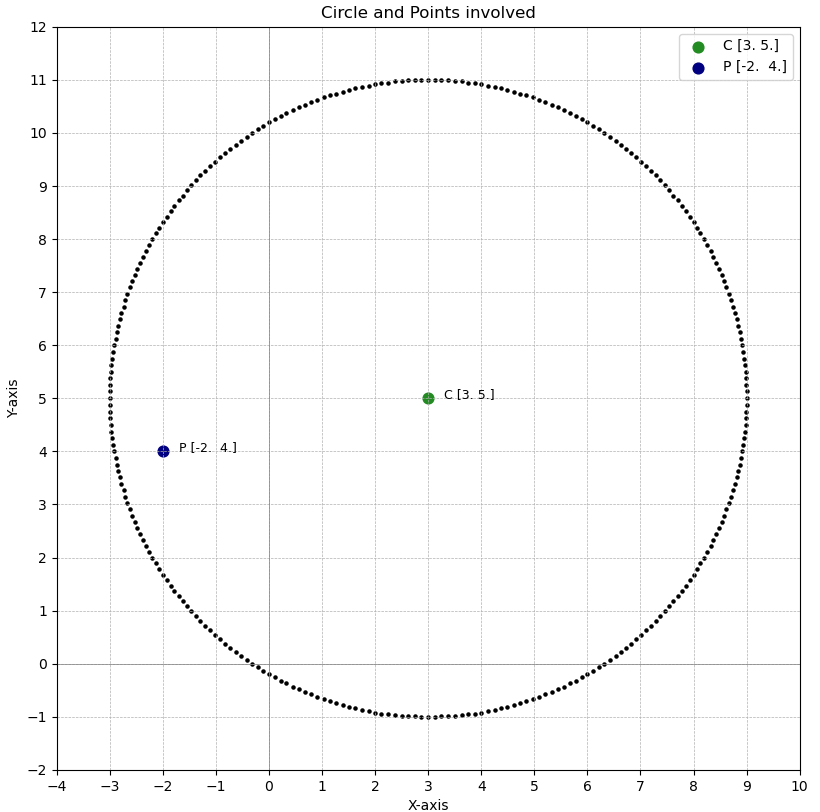
\includegraphics[width=0.7\columnwidth]{figs/Figure_1.png}
    \caption{Circle and Points}
    \label{7-7.2-28-fig-0}
\end{figure}

\end{document}


